% *********************** Це є Розділ 1 ************************************


% \setcounter{chapter}{0}
 \chapter{МОДЕЛЮВАННЯ ФІЗИЧНО ПРАВИЛЬНОЇ ВЗАЄМОДІЇ СВІТЛА ІЗ ПРЕДМЕТАМИ}

 
 \par У цьому розділі наводяться необхідні означення та термінологія, а також висвітлено основні проблеми, пов'язані з моделюванням фізично правильної взаємодії світла з 
      об'єктами в комп'ютерній графіці. 

 \section{Людське сприйняття зображень}
  \setcounter{equation}{0}
 \setcounter{theorem}{0}

 \par Перед тим як вдаватись до деталей моделювання фізично правильної взаємодії світла з об'єктами, важливо розглянути, 
 яким чином людське оке сприй\-має світло та як наш мозок формує остаточне зображення.
 \par Світло -- це квантова елетромагнітна хвиля, швидкість якої становить \break $299\,792\,458\,\text{m/s}$. Видимий спектр світла знаходиться між 
 380 та 780 наномет\-рами (рис. \ref{fig:LightSpectrum}). Видиме світло, яке є монохромним, відповідає деякему кольору спектру. Зазвичай джерела світла випромінюють 
 світло у широкому діапазоні довжин хвиль. Наприклад денне світло є суперпозицією деякого діапазону хвиль (рис. \ref{fig:LightSuper}).
У природі спостерігати це явище можна під час виникнення веселки, коли світло проходить через краплі води, розкладаючись при цьому на спектр кольорів.

 \begin{figure}[h]
  \centering
  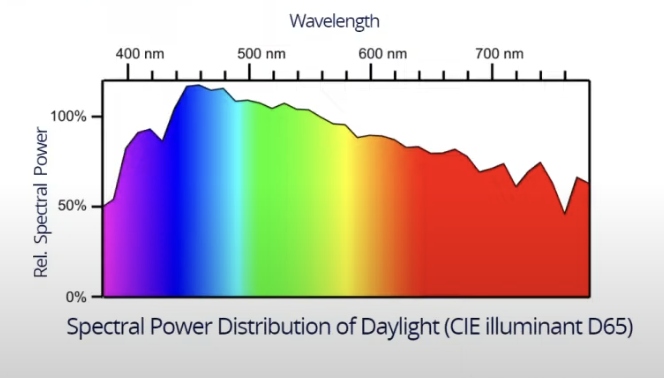
\includegraphics[scale=1]{Pictures/LightSuper.png}
  \caption{Спектральний розподіл енергії денного світла}
  \label{fig:LightSuper}
\end{figure}

\begin{figure}[h]
\centering
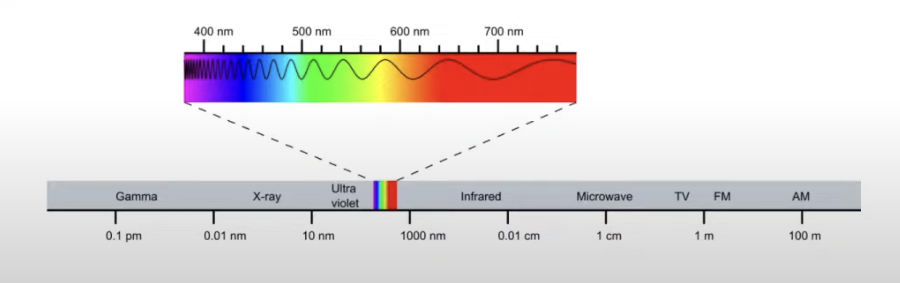
\includegraphics[scale=1]{Pictures/LightSpec.png}
\caption{Видимий спект світла}
\label{fig:LightSpectrum}
\end{figure}

  \par Світло також взаємодіє з навколишніми об'єктами. Припустимо, що світло випромінюється деяким джерелом в однорідних речовинах, наприклад по\-віт\-рі. Оскільки
  рух потоку фотонів є прямолінійним, то деякі промені можуть потрапити одразу в людське око, інші ж -- на об'єкти, які в свою чергу поглинають, відбивають або
  пропускають фотони світла. Відповідно до цього, ми можемо спостерігати різні кольори об'єктів, які залежать від того, які довжини хвиль світла вони відбивають.
  Те світло, яке потрапляє в око людини, проходить через рогівку, кришталик та склоподібне тіло, де воно фокусуються на сітківці ока. Сітківка містить фоторецептори, 
  які реагують на світло і перетворюють його в електричні сигнали, що надсилаються до мозку. Мозок обробляє ці сигнали і формує зображення, яке ми сприймаємо у кінцевому результаті (рис. \ref{fig:LightPath}).

 \begin{figure}[h]
  \centering
  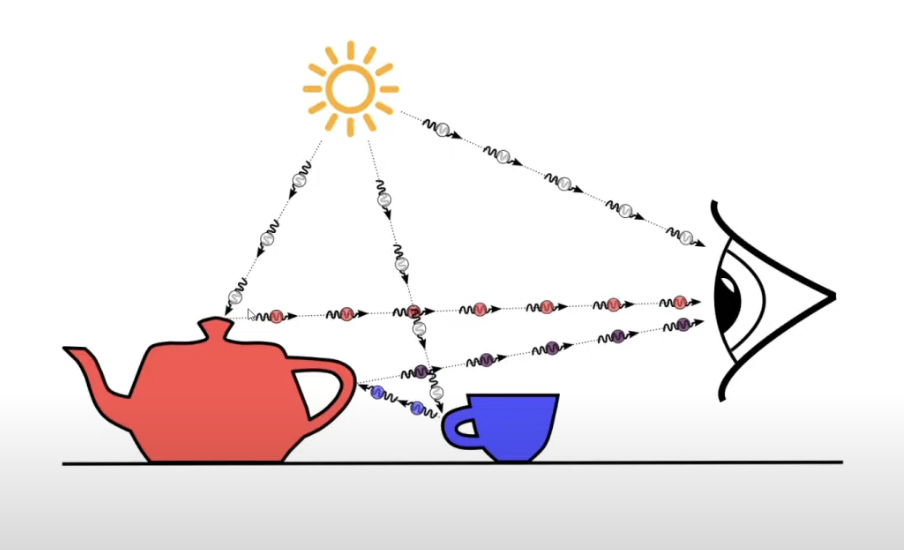
\includegraphics[scale=1]{Pictures/LightPath.png}
  \caption{Шлях світла від джерела до ока людини}
  \label{fig:LightPath}
\end{figure}

\par
Загалом у людини існують дві основні системи фоточутливих рецепторів, що забезпечують зорове сприйняття: палички та колбочки. Розгленемо їх детальніше.
\begin{enumerate}
\item \textbf{Палички} -- фоторецептори, які мають високу чутливість до інтенсивності світла та забезпечують зір при слабкому освітленні 
(скотопічний зір). Вони не розрізняють кольори.
\item \textbf{Колбочки} -- рецептори, відповідальні за кольоровий (фотопічний) зір. Вони чутливі до різних діапазонів довжин хвиль електромагнітного 
випромінювання. Існує три типи колбочок (рис. \ref{fig:LightRecept}):
\begin{enumerate}
    \item \textbf{L-колбочки} (Long) -- реагують на довгі довжини хвиль (при\-близ\-но 560–580 нм), що відповідає червоному діапазону спектра.
    \item \textbf{M-колбочки} (Medium) -- сприймають середні довжини хвиль (при\-близ\-но 530 нм), асоційовані із зеленим кольором.
    \item \textbf{S-колбочки} (Short) -- чутливі до коротких довжин хвиль (при\-близ\-но 420–440 нм), які відповідають синьому кольору.
\end{enumerate}
\end{enumerate}

 \begin{figure}[h]
  \centering
  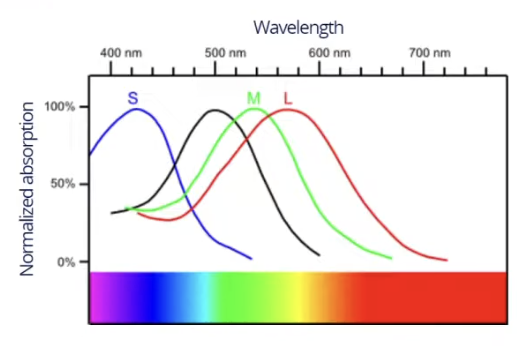
\includegraphics[scale=1]{Pictures/LightRecept.png}
  \caption{Людські колбочки та діапазон їх чутливості}
  \label{fig:LightRecept}
\end{figure}

Через те, що людське око має лише три типи колбочок, воно не може сприй\-ма\-ти реальний спектральний розподіл енергії світла,
завдяки цьому око мож\-на обманювати, і різні спектрані розподіли енергії світла можуть візуалізуватись як однакові кольори. Саме через це, в комп'ютерній графіці
застосовується RGB кольорова модель, де R -- red (червоний), G --green (зелений), B -- blue (синій). Змішуючи ці три кольори в різних пропорціях, можна отримати 
більшість кольорів, які сприймаються людським оком (рис. \ref{fig:RGB}). Прямий фі\-зич\-ний зв'язок між спектральним розподілом енергії світла та RGB описано в \cite{Ch1} та \cite{Ch2}. У контексті комп’ютерної графіки, зокрема при \texit{рендерингу} -- процесі створення фотореалістичного або нефотореалістичного зображення на основі вхідних даних -- це має вирішальне значення.
Більшість сучасних моніторів та екранів використовують sRGB кольорову модель для відображення зображень, але для фізично правильного рендерингу треба працювати в 
лінійному спектрі, для цього застосовується так звана \textit{гамма ко\-рек\-ція}, яка дозволяє перетворити кольори з sRGB в лінійний спектр \cite{Ch5}.
Основна ідея, яку слід засвоїти, полягає в тому, що немає потреби симулювати транспортування світ\-ла для кожної довжини хвилі окремо. Для більшості прак\-тич\-них застосувань 
достатньо розраховувати перенесення світ\-ла для трьох основних кольорів. Це значно спрощує обчислення та робить задачі 
рендерингу обчислювально ефек\-тив\-ні\-ши\-ми.

\begin{figure}[h]
  \centering
  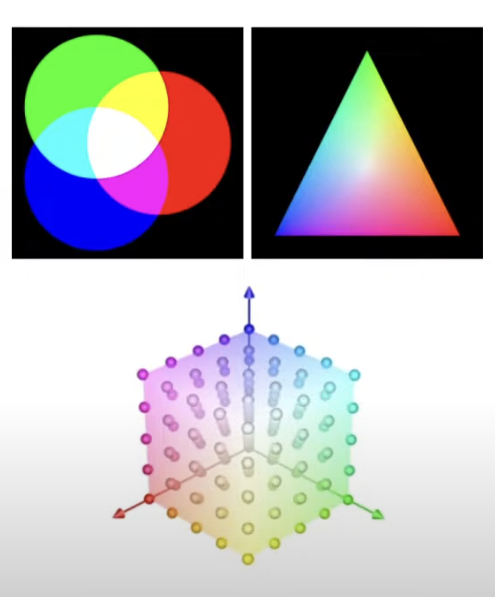
\includegraphics[scale=1]{Pictures/RGB.png}
  \caption{RGB кольорова модель}
  \label{fig:RGB}
\end{figure}

 \section{Визначення рівняння рендерингу}
   \setcounter{equation}{0}
 \setcounter{theorem}{0}

 \subsection{Радіометричні величини} \\

\par
Перш ніж дати визначення рівнянню рендерингу, варто розглянути деякі основні фізичні величини, які в ньому зу\-стрі\-ча\-ють\-ся. Одним із базових понять є \textit{тілесний кут}.

\paragraph{Тілесний кут.}
\par
У шкільній програмі вводиться поняття кута у двовимірному просторі. Щоб визначити, який кут охоплює об’єкт з певної точки спостереження, уявімо коло з центром у цій точці та проектуємо об’єкт на нього. Кут визначається як відношення довжини дуги $s$ до радіуса $r$:
\[
\theta = \frac{s}{r}.
\]
Одиниця плоского кута називається “радіан” (рад) і дорівнює кутові, для якого $s/r=1$.
\par
У тривимірному просторі аналогом звичайного кута є \textit{тілесний кут} (англ. \textit{solid angle}) $\omega$ --  це частина простору, обмежена певною незамкненою конічною поверхнею. 
\par
Щоб визначити тілесний кут, який охоплює об’єкт з певної точки, роз\-міс\-ти\-мо у цій точці центр уявної сфери та спроектуємо об’єкт на її поверхню. Таким чином, тілесний кут визначається як відношення площі проєкції $s$ до квадрата радіуса сфери:
\[
\omega = \frac{s}{r^2}.
\]
Одиницею тілесного кута є стерадіан \textit({sr}),  для якого $\frac{S}{r^2}=1$. Повна сфера має тілесний кут $4\pi$ стерадіан.

\par
Для обчислення тілесного кута, що покриває певну область, необхідно спроектовану область розбити на нескінченно малі елементи $d\omega$ й інтегрувати по всій області:
\[
\omega = \int d\omega.
\]

\par
Зручним способом параметризації є сферичні координати, які задаються двома кутами: полярним $\theta$ (від $0$ до $\pi$) та азимутальним $\phi$ (від $0$ до $2\pi$). Нескінченно мала ділянка тілесного кута виражається через поверхневий елемент $ds$:
\[
d\omega = \frac{ds}{r^2}.
\]
Припускаючи, що радіус $r = 1$, обчислимо $ds$ як площу елемента поверхні сфери:
\[
ds = \sin{\theta} \, d\theta \, d\phi.
\]
Таким чином, фінальна формула для нескінченно малої ділянки тілесного кута набуває вигляду:
\[
d\omega = \sin{\theta} \, d\theta \, d\phi.
\]

А загальна формула для тілесного кута, що охоплює певну область на сфері, виглядає так:
\begin{equation}
\label{eq:SolidAngle}
\omega = \int_0^{2\pi} \int_0^{\pi} \sin{\theta} \, d\theta \, d\phi.
\end{equation}

\paragraph{Потік випромінювання (Radiant Flux).}
\textit{Потік випромінювання} \linebreak (англ. \textit{radiant flux})~$\Phi$, -- це енергія електромагнітного випромінювання, що пе\-ре\-дає\-ть\-ся в одиницю часу:
\[
\Phi = \frac{dQ}{dt},
\]
де $Q$ -- енергія, $t$ -- час. Одиниця вимірювання потоку енергії -- ват (Вт), тобто джоуль на секунду (Дж/с).

Кожен фотон несе енергію, яку можна обчислити за формулою:
\[
E = \frac{hc}{\lambda},
\]
де $h$ -- стала Планка, $c$ -- швидкість світла, $\lambda$ -- довжина хвилі.

Таким чином, потік випромінювання можна інтерпретувати як сумарну енергію фотонів, що випромінюються джерелом світла за одиницю часу. У графіці $\Phi$ 
використовується для опису загального випромінювання точкового джерела.

\paragraph{Інтенсивність випромінювання (Radiant Intensity).}
\textit{Інтенсивність} \linebreak \textit{вип\-ро\-мі\-ню\-ван\-ня} (англ. \textit{Radiant Intensity})  $I$ -- це потік випромінювання на одиницю тілесного кута:
\[
I = \frac{d\Phi}{d\omega}.
\]
Одиниця вимірювання інтенсивності випромінювання -- Вт/ср (ват на стерадіан). Ця величина використовується, коли джерело випромінює світло нерівномірно в різних напрямках, як, наприклад, 
у випадку прожектора. Для точкового джерела, що випромінює рівномірно у всіх напрямках:
\[
I = \frac{\Phi}{4\pi}.
\]

\paragraph{Опроміненість (Irradiance).}
\textit{Опроміненість} (англ. \textit{Irradiance}) $E$ -- це потік випромінювання, що потрапляє на одиницю площі поверхні:
\[
E = \frac{d\Phi}{dA}.
\]
Одиниця вимірювання -- Вт/м$^2$. Потік може надходити з усіх напрямків півсфери над поверхнею. Для нескінченно малої ділянки $dA$, яку 
освітлює точ\-ко\-ве джерело, враховується тілесний кут $d\omega$, під яким джерело можна побачити з цієї ділянки. Якщо $\theta$ -- кут між нормаллю до 
поверхні та напрямком на джерело, то проєкція враховується через множник $\cos{\theta}$:

\[
E = \frac{I \cdot \cos{\theta}}{r^2},
\] де $r$ -- відстань до джерела.

Оскільки $I = \frac{\Phi}{4\pi}$, то для точкового джерела маємо:
\[
E = \frac{\Phi \cdot \cos{\theta}}{4\pi r^2}.
\]

Це показує, що опроміненість зменшується обернено пропорційно до квад\-ра\-та відстані до джерела випромінювання та залежить від кута падіння світла.

\paragraph{Енергетична яскравість (Radiance).}
\texit{Енергетична яскравість} \linebreak (англ. \textit{Radicance}) $L$ визначається як потік випромінювання, що проходить через одиницю площі в певному напрямку, на одиницю тілесного кута:
\[
L = \frac{d^2\Phi}{dA_{\perp} \, d\omega},
\]
де $dA_{\perp} = \cos{\theta} \, dA$ -- проєкція площі в напрямку потоку. Одиниця вимірювання -- $\text{Вт}/(\text{м}^2\cdot\text{ср})$.
Ця величина не залежить від відстані до джерела, адже при зменшенні відстані тілесний кут збільшується, але площа яка спостерігається -- зменшується.
\par
Спостергіти це явище ми можемо на прикладі стіни, змінючи дистанцію до неї, її яскравість 
є сталою.

\paragraph{Зв'язок між опроміненістю та енергетичною яскравістю.}
Опроміненість можна визначити через інтегрування енергетичної яскравості по всій півсфері $\Omega_h$ напрямків над поверхнею:
\begin{equation}
 \label{eq:RadianceToIrradiance}
    E = \int_{\Omega_h} L(\omega) \cos{\theta} \, d\omega.
\end{equation}

\subsection{Рівняння рендерингу} \phantom{Латех просто не скидати текст на новий рядок}
\par Рівняння рендерингу описує, як світло взаємодіє з поверхнями об'єктів і як це впливає на зображення, яке ми бачимо. Воно базується на фізичних принципах 
передачі світла та його взаємодії з матеріалами.
\begin{equation}
\label{eq:RenderingEquation}
  L_o(\vec{v}) = L_e(\vec{v}) + \int_{\Omega_h} f_r(\vec{v},\vec{l} ) L_i(\vec{l}) \cos{\theta} d\omega,
\end{equation} де: $L_o(\vec{v})$ -- вихідна енергетична яскравість у напрямку $\vec{v}$, $L_e(\vec{v})$ -- енер\-ге\-тич\-на яскравість, що випромінюється поверхнею в напрямку $\vec{v}$,
$f_r(\vec{v},\vec{l})$ -- \textit{двопроменева функція розподілу відбивної здатності} (BRDF), що описує, як світло з напрямком $\vec{l}$ відбивається від 
поверхні в напрямок $\vec{v}$, $L_i(\vec{l})$ -- вхідна енер\-ге\-тич\-на яскравість у напрямку $\vec{l}$, 
$\theta$ -- кут між нормаллю до поверхні та напрямком на джерело світла, $d\omega$ -- тілесний кут.
\par
Якщо придивитися уважно, то можна побачити, що рівняння рендерингу \ref{eq:RenderingEquation} містить в собі рівняння для опроміненості \eqref{eq:RadianceToIrradiance}. Інакше кажучи, рівняння \ref{eq:RenderingEquation} описує, що саме побачить спостерігач у напрямку $\mathbf{-v}$, дивлячись на точку, яка сама 
випромінює світло у напрямку $\vec{v}$ та додатково опромінюється іншими об'єктатами, розташованих на уявній півсфері, що охоплює цю точку.

\paragraph{Складність обчислення рівняння освітлення.}

Інтегрування по всій півсфері напрямків~$\Omega_h$ означає врахування всіх можливих напрямків по\-ши\-рен\-ня світла, яке може впливати на задану точку поверхні.
Це робить рівняння освітлення обчислювально складним, адже для кожної точки сцени потрібно проінтегрувати внесок світла з усіх напрямків півсфери, орієнтованої відносно нормалі до поверхні.
Під \textit{сценою} у комп’ютерній графіці розуміють сукупність усіх візуальних елементів -- геометрії, матеріалів, джерел світла та камери -- які разом утворюють просторову конфігурацію, що підлягає візуалізації.

Кожен об’єкт у сцені сам по собі є джерелом випромінювання, тобто володіє певною вихідною енергетичною яскравістю в довільному напрямку~$\vec{v}$. Взаємне 
освітлення між об’єктами створює глобальну взаємозалежність, де світ\-ло, відбите від однієї поверхні, може впливати на інші поверхні, і так далі -- потенційно нескінченну
 кількість разів.

Складність посилюється тим, що будь-яка поверхня є зв'язною\footnote{Кількість світлових променів у сцені є скінченними, проте їхня кількість настільки велика, що доречно вважати їх нескінченними} множиною точок, а з кожної точки в нескінченну кількість напрямків можуть надходити фотони. На 
локальому рівні поверхні не ідеально гладкі: вони можуть мати шорсткості, мікрогеометрію, відмінні оптичні властивості (наприклад, металічність, діелектричність,
 шорсткість тощо), що впливає на спосіб взаємодії зі світлом.

Оскільки світло може багаторазово відбиватися між поверхнями перед тим, як потрапити в камеру або око спостерігача, то точне симулювання всіх траєкторій кожного 
фотона є обчислювально недосяжним\footnote{Слід зауважити, що існують методи, такі як Ray Tracing та Path Tracing, які симулюють поведінку світла, але лише для скінченної кількості променів, та
малої кількість відбитів світла від поверхонь} завданням для су\-час\-них комп’ютерів.

У зв’язку з цим, замість точного моделювання всіх траєкторій, у комп’ю\-тер\-ній графіці застосовуються стохастичні методи, які описують розповсюдження світла у вигляді
 ймовірнісного процесу. Зокрема, розглядається ймовірність того, що промінь світла з певного напрямку~$\vec{l}$, взаємодіючи з поверхнею з відомими матеріальними 
 властивостями, буде відбитий в інший напрямок або поглинутий. Саме BRDF функція дозволяє моделювати цю ймовірність, і давати загальне уявлення про те, як світло
взаємодіє з поверхнею.

\subsection{BRDF та його роль у моделюванні відбиття світла}
\phantom{Латех...}
\par BRDF (Bidirectional Reflectance Distribution Function -- двонаправлена функ\-ція розподілу відбиття) -- це чотиривимірна функція, якщо не враховувати залежність 
від довжини хвилі. Саме вона точно описує відбивні властивості поверхні. BRDF певного матеріалу можна виміряти експериментально й зберігати у вигляді 4D-таблиці. 
Однак такий підхід потребує великої кількості пам'яті та ускладнює редагування матеріалів. Тому у більшості випадків використовують параметричні моделі BRDF, як-от 
модель Фонга чи модель Бліна-Фонга \cite{Ch3}.
\par У комп'ютерній графіці також застосовується поняття мікрофасетів -- це дрібні ділянки поверхні, розмір яких набагато менший за піксель. 
Передбачається, що кожен мікрофасет поводиться як ідеальне дзеркало, а їх орієнтації розподілені за певним статистичним законом розподілу навколо мікро\-ско\-піч\-ної нормалі поверхні. Через ці відхилення від ідеальної нормалі світло відбивається не в одному напрямку, а розсіюється навколо напрямку ідеального відбиття.
Чим вища шорсткість поверхні, тим більший розмах розподілу відбитого світла. Для металів фотони або відбиваються, або поглинаються всередині матеріалу -- залежно від 
довжини хвилі. Через це відбите світло може мати певний колір, як у випадку з  міддю чи золотом. Така поведінка характерна саме для металів.У діелектриків 
(неметалевих матеріалів) модель відбиття інша, ніж у металів. Частина фотонів також відбивається від поверхні -- це так зване дзеркальне відбиття (specular reflection). 
Але на відміну від металів, це відбиття не залежить від довжини хвилі, тому воно не має кольору. Решта фотонів проникає в матеріал, де або поглинається, 
або розсіюється під поверхнею в довільних напрямках. Частина з них зрештою виходить назад з поверхні -- це явище називається дифузним відбиттям (diffuse reflection). Воно залежить від довжини хвилі, а отже, для діелектриків є кольоровим.
\par
Єдиного вигляду у функції BRDF нема, адже це сімейство функцій які задаються формулою:
\begin{equation}
\label{eq:BRDF_DS}
f_r = f_d + f_s,
\end{equation}
де $f_d$ -- це дифузне відбиття, а $f_s$ -- дзеркальне відбиття, та повинні задовольняти низку фізичних властивостей:

\begin{enumerate}
    \item \textbf{Невід’ємність:} BRDF ніколи не повинна генерувати від'ємне зна\-чен\-ня, адже від'ємної енергетичної яскравості не існує.

    \item \textbf{Реципрокність (взаємність) за Гельмгольцем:} Зна\-чен\-ня BRDF повинне залишатися незмінним при перестановці 
    напрямків спостереження $\vec{v}$ і освітлення $\vec{l}$, тобто:
    \[
    f_r(\vec{v}, \vec{l}) = f_r(\vec{l}, \vec{v}).
    \]
    Це означає, що освітлення сцени і її спостереження повинні бути симетричними по відношенню до розподілу світлового потоку.

    \item \textbf{Закон збереження енергії:} BRDF повинна також дотримуватися принципу збереження енергії. Якщо розглянути другу частину рів\-нян\-ня 
    \ref{eq:RenderingEquation}, яка описує інтегрування опроміненості по напівсфері $\Omega$, та припустити, що вхідна опроміненість з усіх напрямків дорівнює 1, 
    то енергетична яскравість не може перевищувати цього зна\-чен\-ня:
    \[
    \int_{\Omega} (f_d(\vec{v}, \vec{l}) + f_s(\vec{v}, \vec{l})) \cdot\cos\theta \, d\omega \leq 1.
    \]
    Значення, менше за 1, є фізично допустимим, оскільки частина світ\-ла може бути поглинена матеріалом і перетворена, наприклад, у теп\-ло. 
    Проте значення, що перевищують 1, порушують закон збереження енергії та вказують на некоректність BRDF, адже у такому випадку модель фактично створює нову 
    енергію, що є неможливим при прос\-то\-му відбитті світла.
\end{enumerate}